\chapter{Introdução}

Sistemas embarcados estão presentes em uma ampla gama de aplicações, que vão desde dispositivos médicos e sistemas de automação industrial
até plataformas automotivas e missões espaciais. Diferentemente da computação de propósito geral, esses sistemas operam sob rigorosos requisitos
temporais, nos quais a corretude do comportamento não depende apenas da precisão lógica dos resultados produzidos, mas também do momento
exato em que esses resultados são disponibilizados. Em muitos casos, atrasos mínimos ou falhas temporais podem comprometer a segurança, a
confiabilidade e até mesmo a integridade física de pessoas e equipamentos.

Tradicionalmente, a garantia desse determinismo esteve associada ao uso de plataformas dedicadas, nas quais \glspl{rtos} são empregados para assegurar
previsibilidade temporal, isolamento entre tarefas e cumprimento de restrições rígidas de escalonamento. Entretanto, a evolução do software contemporâneo
deslocou grande parte dos ecossistemas de desenvolvimento — bibliotecas, frameworks, ferramentas e serviços — para ambientes baseados em \glspl{gpos} - 
especialmente Linux. Embora esses sistemas ofereçam grande riqueza funcional e amplo suporte da comunidade, sua adoção em contextos críticos embarcados demanda
esforços adicionais de adaptação, validação e integração.

Como resultado, cresce a necessidade de consolidar, em uma mesma plataforma computacional, cargas de trabalho com requisitos distintos e frequentemente
conflitantes: de um lado, aplicações críticas, sensíveis a prazos temporais e dependentes de comportamento determinístico; de outro, aplicações complexas,
orientadas a funcionalidades avançadas e dependentes de ambientes generalistas.

Nesse cenário, técnicas de virtualização surgem como uma alternativa promissora, pois permitem a coexistência de múltiplos ambientes de execução sobre o
mesmo hardware. Dessa forma, torna-se possível executar aplicações críticas e não críticas de maneira controlada, reduzindo custos de integração e
aumentando o aproveitamento da plataforma.

Paralelamente, a arquitetura aberta RISC-V destaca-se por sua flexibilidade, modularidade e ausência de barreiras proprietárias, impulsionando o desenvolvimento de soluções customizadas e de
baixo custo. Contudo, esses processadores mais simples raramente dispõem de extensões de hardware dedicadas à virtualização. Esse cenário gera um gargalo relevante, visto que a maioria das
plataformas de virtualização atuais depende estritamente desses recursos físicos para funcionar.

Por isso, este trabalho propõe o projeto e a implementação, em C++, de uma infraestrutura de virtualização voltada a sistemas embarcados
baseados em RISC-V. A proposta tem como foco a previsibilidade temporal, o isolamento entre cargas de trabalho, o reduzido custo de execução e a possibilidade de utilização em plataformas de recursos
computacionais limitados. Busca-se, dessa forma, contribuir para o desenvolvimento de plataformas embarcadas capazes de executar, de forma simultânea e isolada, cargas de trabalho heterogêneas,
conciliando requisitos de desempenho, determinismo temporal e confiabilidade.

\section{Objetivos}

\subsection{Objetivos Gerais}

Desenvolver e avaliar uma infraestrutura de virtualização em C++ para sistemas embarcados baseados na arquitetura RISC-V,
focada no particionamento estático de recursos, no isolamento de cargas de trabalho de criticidade mista e na garantia da previsibilidade temporal para aplicações de tempo real.

\subsection{Objetivos Específicos}

\begin{itemize}
    \item Projetar e implementar em software o núcleo do hipervisor para o gerenciamento, criação, inicialização e execução de máquinas virtuais em plataformas RISC-V\@;
    \item Implementar o particionamento estático de processadores, memória e dispositivos de \gls{io}, garantindo o isolamento espacial e temporal entre domínios;
	\item Validar a infraestrutura funcionalmente por meio da execução de \glspl{so} convidados representativos;
	\item Quantificar o impacto do hipervisor no desempenho do sistema, mensurando \textit{overheads} computacionais e a previsibilidade temporal sob restrições de tempo real.
\end{itemize}

\chapter{Fundamentação Teórica}

\section{Sistemas Embarcados}

Sistemas embarcados são soluções computacionais projetadas para executar funções dedicadas no interior de equipamentos maiores. Amplamente utilizados em setores como automação industrial,
indústria automotiva, medicina, telecomunicações e \gls{iot}, esses sistemas destacam-se pela forte integração entre hardware e software. Como operam frequentemente sob restrições severas de
processamento, memória, armazenamento e consumo de energia, exigem um desenvolvimento altamente otimizado para entregar máxima eficiência com baixo custo computacional.

\section{Sistemas Operacionais}

Um sistema operacional é um software responsável por gerenciar os recursos de hardware de um sistema computacional e fornecer serviços para a execução de aplicações.
Atuando como uma camada de abstração entre o hardware e os programas, o sistema operacional simplifica o desenvolvimento de software ao oferecer mecanismos padronizados
para acessar o processador, memória, dispositivos de entrada e saída, dispositivos armazenamento de dados, etc.

A evolução dos sistemas operacionais permitiu o surgimento de plataformas cada vez mais complexas, capazes de executar múltiplas aplicações simultaneamente e
fornecer diversos serviços ao usuário. Entretanto, dependendo dos requisitos da aplicação, características como previsibilidade temporal, confiabilidade e isolamento podem
se tornar tão importantes quanto o desempenho, motivando o desenvolvimento de sistemas operacionais especializados.

\section{Sistemas De Tempo Real}

Sistemas que operam sob restrições de tempo real são sistemas nos quais a reatividade temporal é extremamente importante para a corretude ou até mesmo para a
segurança do ambiente de execução. Nesses sistemas, não é suficiente que uma operação produza um resultado correto ou que seja extremamente rápida, sendo também necessário que esse resultado
seja produzido dentro de um intervalo de tempo determinado \cite{stankovic1988misconceptions}. 

Para atender a esses requisitos, são empregados \glspl{rtos}, projetados para fornecer mecanismos de gerenciamento de tarefas e recursos que favoreçam a previsibilidade e o cumprimento de
restrições temporais. Diferentemente de \glspl{gpos}, nos quais o objetivo principal geralmente está relacionado ao aumento do desempenho médio, da utilização dos
recursos ou da responsividade percebida pelo usuário, um \gls{rtos} prioriza a capacidade de determinar e controlar os tempos envolvidos na execução das tarefas.

Os conceitos centrais associados aos \glspl{rtos} são o \textit{deadline} e o determinismo. O \textit{deadline} - ou prazo limite - refere-se ao instante máximo em que a execução de uma
determinada tarefa deve ser concluída, cabendo ao \gls{rtos} gerenciar os recursos para assegurar o cumprimento desta restrição. Por sua vez, o determinismo — frequentemente associado
à previsibilidade do sistema — garante que o comportamento temporal do software seja conhecido e limitado, com a determinação do tempo de execução no pior caso ou \gls{wcet}.

O elemento central do núcleo de um \gls{rtos} que viabiliza essa previsibilidade é o algoritmo de escalonamento de tarefas  - adaptado para tempo real.
Entre os algoritmos mais consolidados na literatura, destacam-se o \gls{edf}, utilizado em cenários com prioridades dinâmicas — nos quais o conjunto de tarefas ou seus prazos podem
variar em tempo de execução —, e o \gls{rm}, voltado a cenários estáticos, onde as tarefas e seus períodos de ativação são totalmente conhecidos em fase de projeto.

\subsection{Classificação De Sistemas De Tempo Real}

Tais sistemas são classificados de acordo com as consequências do não cumprimento dos requisitos temporais definidos em sua elaboração.
Sistemas nos quais a perda de um prazo pode causar danos catastróficos, como a perda de vidas humanas ou a destruição de equipamentos de alto valor, são classificados como Hard Real-Time.
Por outro lado, sistemas nos quais o atraso temporal não é desejável, mas também não é fatal ou crítico — como o atraso na entrega de quadros em serviços de vídeo —, são chamados de Soft Real-Time.

\subsection{Outros Aspectos De Previsibilidade Temporal}

\begin{itemize}
    \item \textbf{Latência:} intervalo de tempo entre a ocorrência de um evento e o início da ação correspondente do sistema.

    \item \textbf{\textit{Jitter}:} variação temporal observada na latência ou no instante de ocorrência de eventos em relação ao comportamento esperado.

    \item \textbf{\textit{Overhead}:} custo computacional adicional introduzido por algum mecanismo.
\end{itemize}




\section{Virtualização}

Virtualização é uma técnica computacional que permite a execução simultânea e isolada de múltiplos \glspl{so} — denominados sistemas convidados — em um mesmo hardware físico.
Enquanto um \gls{so} convencional atua como uma interface entre o usuário e a máquina, abstraindo a complexidade da arquitetura subjacente, existem sistemas projetados
para estender essa abstração a outros \glspl{so}. Esses sistemas são denominados hipervisores, e o mecanismo que viabiliza esse processo é chamado de virtualização.

De modo geral, existem dois principais tipos de virtualização: a virtualização completa e a paravirtualização.

Na virtualização completa, também conhecida como \textit{full virtualization}, o \gls{so} convidado executa sem ter conhecimento explícito de que está em um ambiente virtualizado.
Nesse cenário, operações privilegiadas são interceptadas pelo hipervisor por meio de exceções e tratadas por mecanismos como \textit{trap-and-emulate}.
Entretanto, esse processo pode comprometer o desempenho do sistema, devido ao custo associado às operações de salvamento e restauração de contexto realizadas a cada exceção gerada.

Em contraste, a paravirtualização adota uma abordagem cooperativa entre o \gls{so} convidado e o seu hipervisor.
Nesse modelo, o sistema convidado é modificado para reconhecer a presença do ambiente virtualizado e, em vez de executar diretamente instruções privilegiadas,
realiza chamadas explícitas ao hipervisor, conhecidas como \textit{hypercalls}. Essa estratégia reduz a necessidade de exceções, diminuindo o custo associado ao processo de virtualização.

\section{Interceptação e Emulação}

Do inglês \textit{trap-and-emulate}, interceptação e emulação trata-se de um método utilizado para viabilizar a virtualização em sistemas nos quais o suporte de
hardware não é completamente implementado. Nesse modelo, quando a aplicação executada em ambiente virtualizado tenta realizar uma operação que depende de recursos privilegiados,
essa operação é interceptada e tratada como uma exceção. O controle é então transferido para um nível mais privilégiado, geralmente o hipervisor, que fica responsável por
emular em software o comportamento esperado da instrução ou operação originalmente solicitada.

\begin{figure}[H]
\centering
\includegraphics[width=0.8\textwidth]{images/TrapAndEmulate.pdf}
\caption{Fluxograma de Interceptação de Instruções Privilegiadas}\label{fig:trap-and-emulate}
\end{figure}



\section{\textit{VirtIO}}

\textit{VirtIO} \cite{Rusty-Russell-VirtIO} é um padrão para drivers de dispositivos paravirtualizados, projetado para unificar e otimizar a interface de comunicação entre os
sistemas convidados e o hipervisor. Em vez de emular hardwares legados complexos e específicos, o hipervisor expõe uma série de dispositivos virtuais padronizados, permitindo que
o \gls{so} convidado acesse recursos de rede, armazenamento e console de maneira eficiente e com baixa sobrecarga.

Para viabilizar essa comunicação, o modelo utiliza as chamadas \textit{Virtqueues} — filas circulares compartilhadas responsáveis pelo envio e recebimento das requisições.
Dependendo das operações suportadas, cada dispositivo virtual pode alocar uma ou mais dessas filas. Internamente, uma \textit{Virtqueue} divide-se em três componentes principais:
uma tabela de descritores (\textit{Descriptor Table}), um anel de índices disponíveis (\textit{Available Ring}) e um anel de índices já utilizados (\textit{Used Ring}).

Na prática, o ciclo de vida de uma operação de \gls{io} ocorre em duas etapas complementares. Inicialmente, quando o sistema convidado deseja realizar uma operação, o dispositivo \textit{VirtIO}
escreve os dados na memória compartilhada, insere o descritor correspondente no \textit{Available Ring} e notifica o hipervisor sobre a nova pendência. 

Em resposta, o hipervisor consome os descritores desse anel, processa a operação solicitada e registra o resultado no \textit{Used Ring}. Por fim, uma interrupção
é enviada ao sistema convidado para sinalizar a conclusão da tarefa. Graças a esse design, múltiplas requisições podem ser tratadas de maneira assíncrona e em lote, o que minimiza
as trocas de contexto e reduz expressivamente o custo inerente à virtualização.

Desse modo, o \textit{VirtIO} consolida-se como uma solução fundamental para a infraestrutura de virtualização moderna, pois alcança um equilíbrio entre a flexibilidade de uma interface padronizada e o
desempenho da paravirtualização.

\section{Hipervisors}

Um hipervisor, também conhecido como \gls{vmm}, é uma plataforma que cria e executa máquinas virtuais via virtualização.
Segundo \citeonline{PopekGeraldGoldberg} um \gls{vmm} possuí três características essenciais: primeiro, devem fornecer um ambiente idêntico à máquina original
para programas; segundo, os programas executados nesse ambiente, na pior das hipóteses, devem apresentar no máximo pequenas reduções
de velocidade que urgem da camada de virtualização; e por último, os \glspl{vmm} devem deter o contole total sobre os recursos do sistema.

Na visão de \cite{Goldberg}, fundamentalmente, existem dois tipos de hipervisores: 1 e 2.

\subsection{Tipo 1 - Bare Metal}

Hipervisores de tipo 1, também conhecidos como bare metal, são aqueles que executam diretamente sobre o hardware físico, sem a necessidade de um
sistema operacional hospedeiro intermediário.
Por operar diretamente sobre o hardware, esse tipo de hipervisor geralmente apresenta melhor desempenho e menor sobrecarga.

\begin{figure}[H]
    \centering
    \begin{tikzpicture}[
        pequeno/.style={
            draw,
            thick,
            fill=blue!5,
            minimum width=4cm,
            minimum height=1.2cm,
            outer sep=0pt
        }
    ]
        \node[pequeno] (apps-so1-1) {Aplicação 1};
        \node[pequeno, right=0.2cm of apps-so1-1] (apps-so1-2) {Aplicação 2};
        \node[pequeno, right=0.2cm of apps-so1-2] (apps-so2-1) {Aplicação 1};

        \node[fit=(apps-so1-1)(apps-so1-2), inner sep=0pt] (apps-so1) {};
        \node[fit=(apps-so2-1), inner sep=0pt] (apps-so2) {};

        \node[
            draw,
            thick,
            fill=blue!10,
            minimum width=8.2cm,
            minimum height=1.5cm,
            below=0.2cm of apps-so1
		] (SO1) {\Gls{so} 1};

		\node[
            draw,
            thick,
            fill=blue!10,
            minimum width=4cm,
            minimum height=1.5cm,
            below=0.2cm of apps-so2
		] (SO2) {\Gls{so} 2};

		\node[fit=(SO2)(SO1), inner sep=0pt] (SOs) {};

		\node[
            draw,
            thick,
            fill=blue!15,
            minimum width=12.4cm,
            minimum height=1.5cm,
            below=0.2cm of SOs
		] (HOS) {Hipervisor};

		\node[
            draw,
            thick,
            fill=blue!20,
            minimum width=12.4cm,
            minimum height=1.5cm,
            below=0.2cm of HOS
		] () {Hardware};

    \end{tikzpicture}
    \caption{Hipervisor Tipo 1.}
    \label{fig:hypervisor-type-1}
\end{figure}

\subsection{Tipo 2}

Diferentemente da solução bare metal, um hipervisor do tipo 2 é executado como um processo dentro de um \gls{so} hospedeiro.
Porém, apesar de garantir os mesmos recursos do tipo 1, sua arquitetura impõe uma camada intermediária a mais de software, o que restringe a
eficiência no acesso aos componentes físicos, gerando uma latência adicional e um menor desempenho.

\begin{figure}[H]
    \centering
    \begin{tikzpicture}[
        pequeno/.style={
            draw,
            thick,
            fill=blue!5,
            minimum width=4cm,
            minimum height=1.2cm,
            outer sep=0pt
        }
    ]
        \node[pequeno] (apps-so1-1) {Aplicação 1};
        \node[pequeno, right=0.2cm of apps-so1-1] (apps-so1-2) {Aplicação 2};
        \node[pequeno, right=0.2cm of apps-so1-2] (apps-so2-1) {Aplicação 1};

        \node[fit=(apps-so1-1)(apps-so1-2), inner sep=0pt] (apps-so1) {};
        \node[fit=(apps-so2-1), inner sep=0pt] (apps-so2) {};

        \node[
            draw,
            thick,
            fill=blue!10,
            minimum width=8.2cm,
            minimum height=1.5cm,
            below=0.2cm of apps-so1
		] (SO1) {\Gls{so} 1};

		\node[
            draw,
            thick,
            fill=blue!10,
            minimum width=4cm,
            minimum height=1.5cm,
            below=0.2cm of apps-so2
		] (SO2) {\Gls{so} 2};

		\node[fit=(SO2)(SO1), inner sep=0pt] (SOs) {};

		\node[
            draw,
            thick,
            fill=blue!15,
            minimum width=12.4cm,
            minimum height=1.5cm,
            below=0.2cm of SOs
		] (HOS) {Hipervisor};

		\node[
            draw,
            thick,
            fill=blue!20,
            minimum width=12.4cm,
            minimum height=1.5cm,
            below=0.2cm of HOS
		] (OS) {\Gls{so}};

		\node[
            draw,
            thick,
            fill=blue!25,
            minimum width=12.4cm,
            minimum height=1.5cm,
            below=0.2cm of OS
		] () {Hardware};

    \end{tikzpicture}
    \caption{Hipervisor Tipo 2.}
    \label{fig:hypervisor-type-2}
\end{figure}

\section{RISC-V}

A RISC-V é uma \gls{isa} baseada nos princípios \gls{risc}. Diferentemente de arquiteturas proprietárias,
a RISC-V possui uma especificação aberta e livre de \textit{royalties}, o que permite sua utilização tanto em contextos acadêmicos quanto em aplicações
comerciais.

Essa \gls{isa} define um conjunto básico de instruções, responsável pelas funcionalidades essenciais do processador. No entanto, sua
principal característica é a modularidade, permitindo que diferentes extensões sejam incorporadas conforme as necessidades da plataforma.
Dessa forma, é possível adaptar a arquitetura para cenários variados, desde sistemas embarcados com restrições de recursos até sistemas de
alto desempenho.

\subsection{Extensões Básicas}

\begin{description}

\item[I]
Adiciona suporte às instruções básicas de operações com números inteiros. Conforme descrito em~\cite{isa-riscv}, essa extensão deve estar
presente em qualquer implementação RISC-V, pois define as operações fundamentais de aritmética e manipulação de registradores.

\item[Zicsr]
Adiciona suporte às instruções de acesso e manipulação de \glspl{csr}.

\item[H]
Adiciona suporte ao modo H (Hipervisor).

\item[S]
Adiciona suporte ao modo S (Supervisor).

\item[M]
Adiciona suporte a operações de multiplicação e divisão de números inteiros.

\item[A]
Adiciona suporte a operações atômicas em memória.

\item[F]
Adiciona suporte a números em ponto flutuante de precisão simples (32 bits).

\item[D]
Adiciona suporte a números em ponto flutuante de precisão dupla (64 bits).

\item[C]
Adiciona suporte a instruções comprimidas de 16 bits.

\item[V]
Adiciona suporte a operações vetoriais para \gls{simd}.

\item[B]
Adiciona suporte à manipulação de bits em hardware, otimizando operações bit a bit.

\item[G]
Aglomerado geral de extensões (*General Purpose*) que inclui I, M, A, F, D e as extensões de controle Zicsr e Zifencei.

\end{description}

\subsection{Níveis de Privilégio}

Assim como a maior parte das arquiteturas modernas, a RISC-V utiliza um modelo hierárquico de privilégios para garantir a segurança e a estabilidade do sistema.
Esses níveis determinam quais operações e recursos de hardware podem ser acessados em cada contexto de execução. Os modos implementados em uma plataforma dependem
diretamente das extensões suportadas, estruturando-se tipicamente em três cenários principais:

\begin{itemize}

\item \textbf{Sem a extensão S:} Utiliza apenas o modo \textit{Machine} e o modo \textit{User}, indicado para sistemas embarcados mais simples e sem suporte a sistemas operacionais baseados em supervisor.
    \begin{figure}[H]
    \centering
    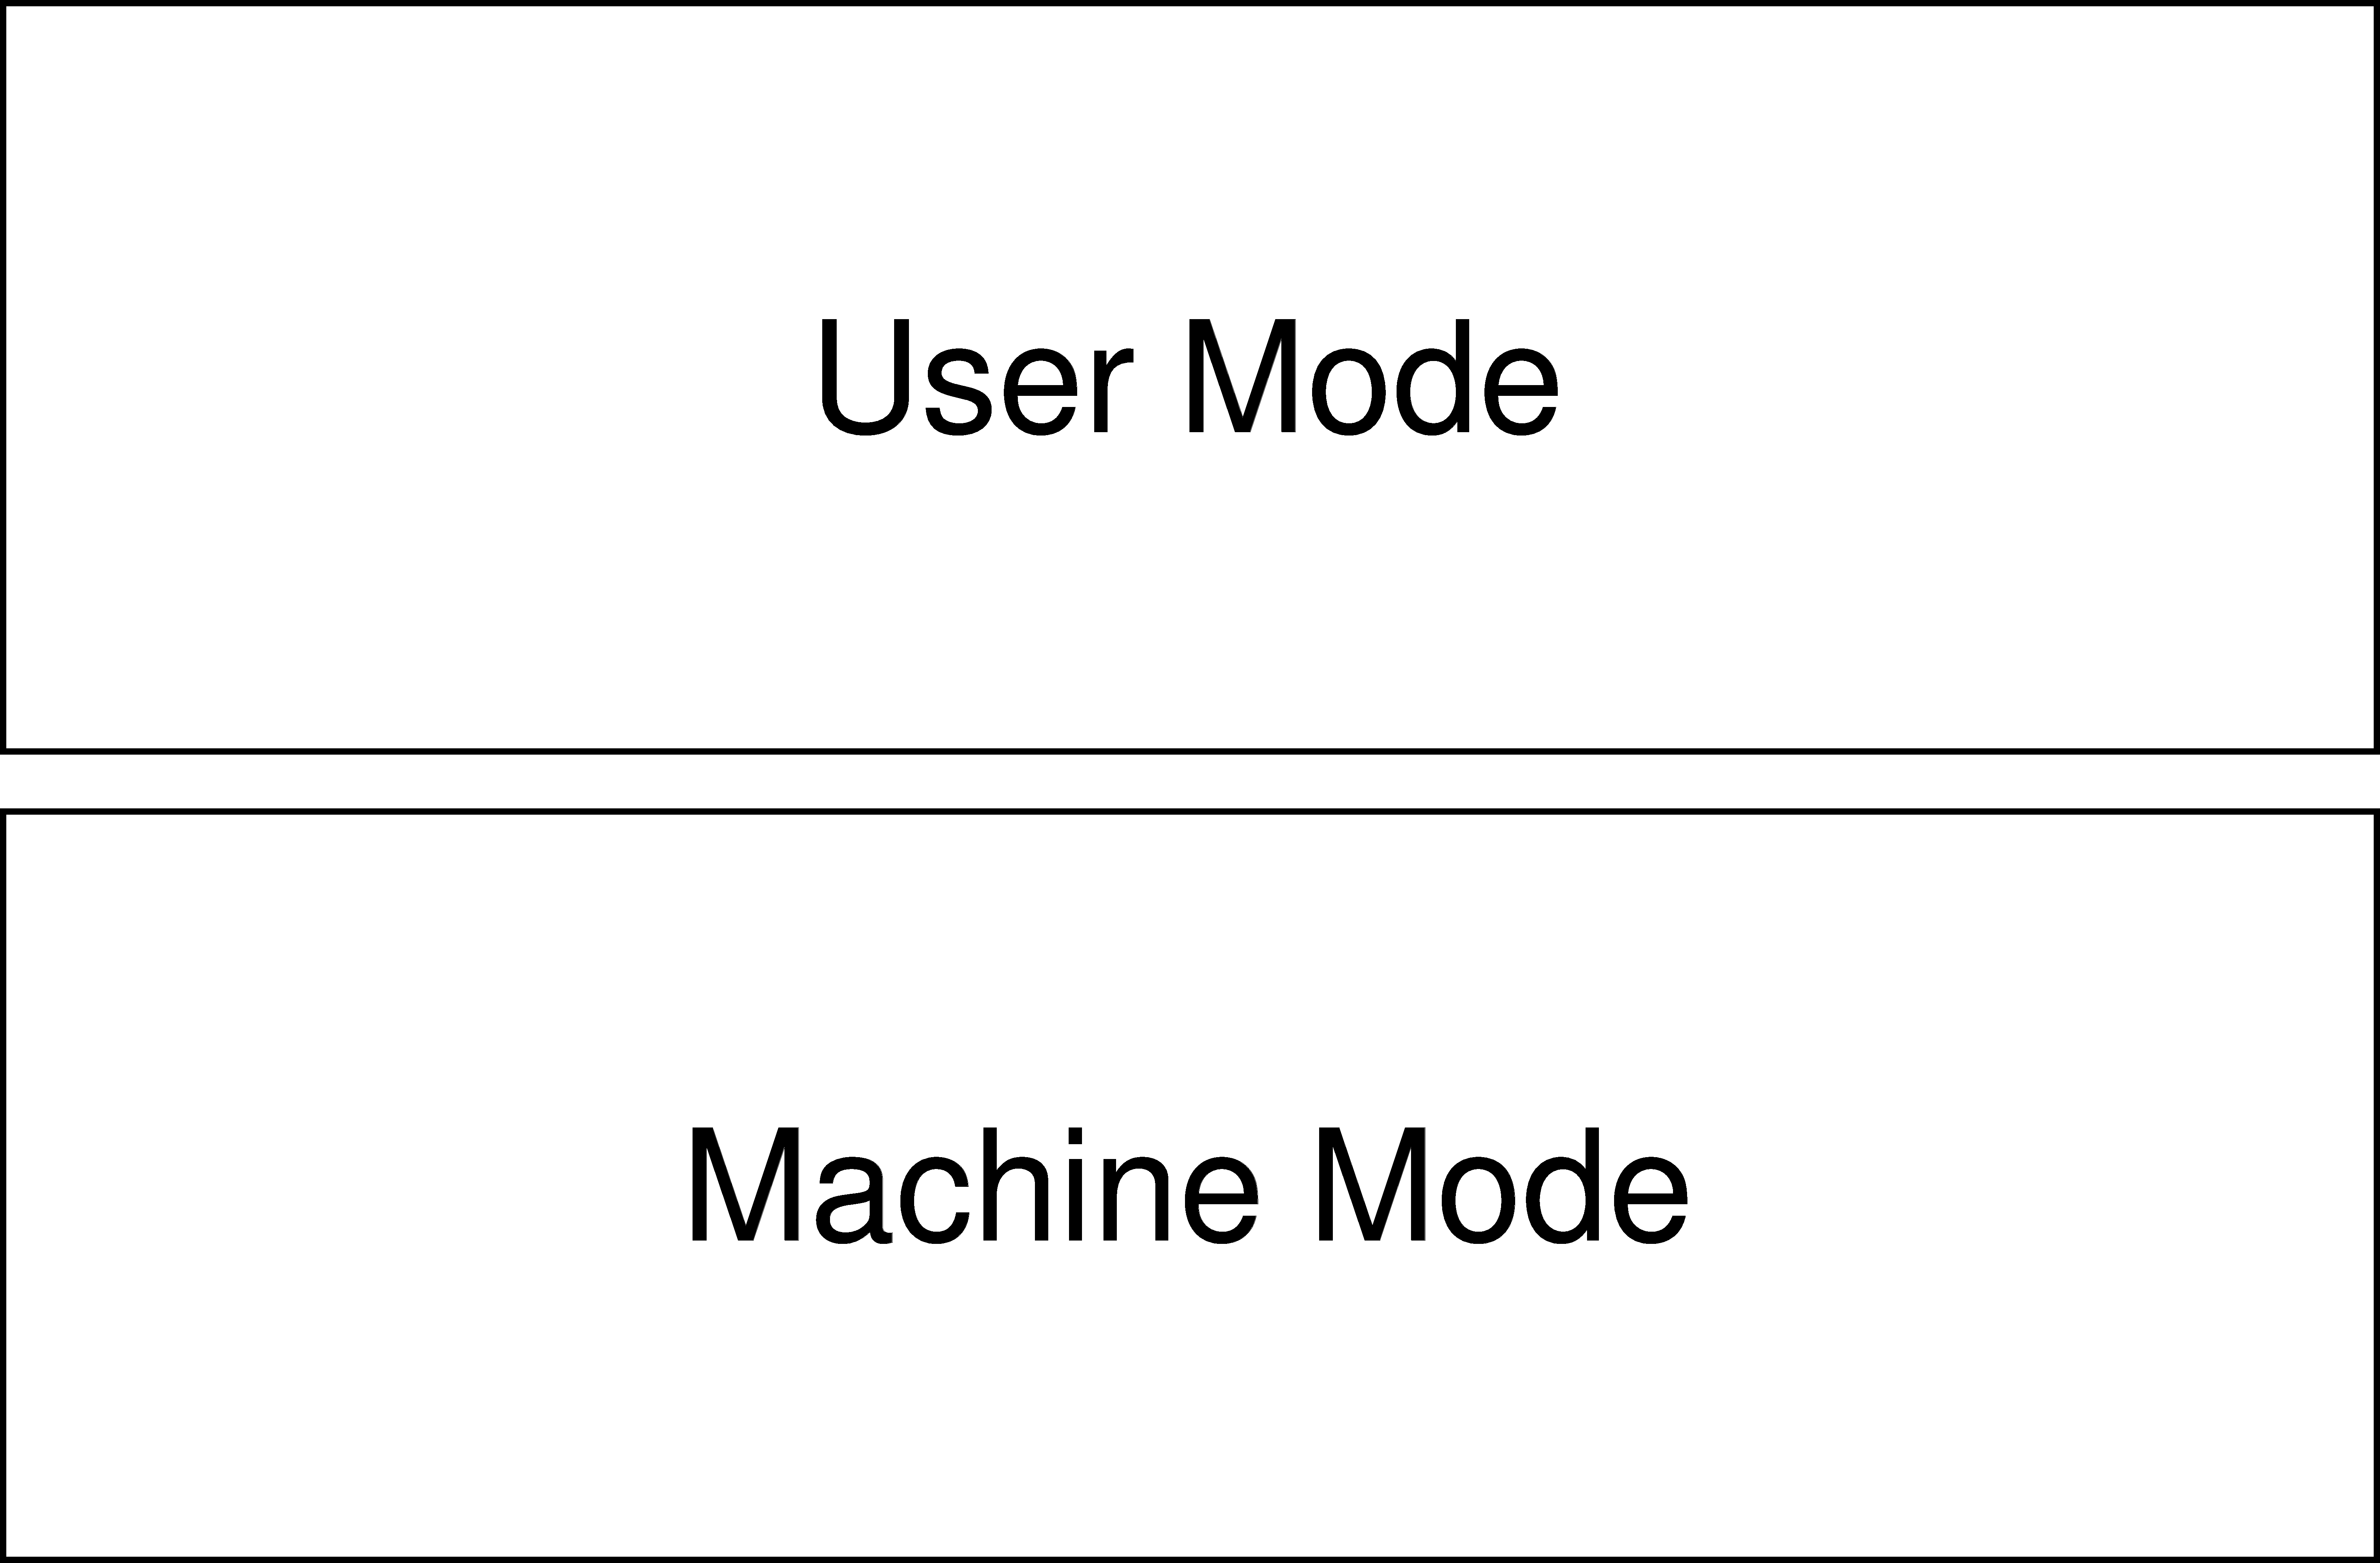
\includegraphics[width=0.3\textwidth]{images/MachineModeUserMode.pdf}
    \caption{Arquitetura de Privilégios RISC-V Sem Modo Supervisor}\label{fig:machine-mode-user-mode}
    \end{figure}

\item \textbf{Com a extensão S:} Adiciona o modo \textit{Supervisor}, permitindo a execução de sistemas operacionais completos que exigem isolamento entre o kernel e as aplicações de usuário.
    \begin{figure}[H]
    \centering
    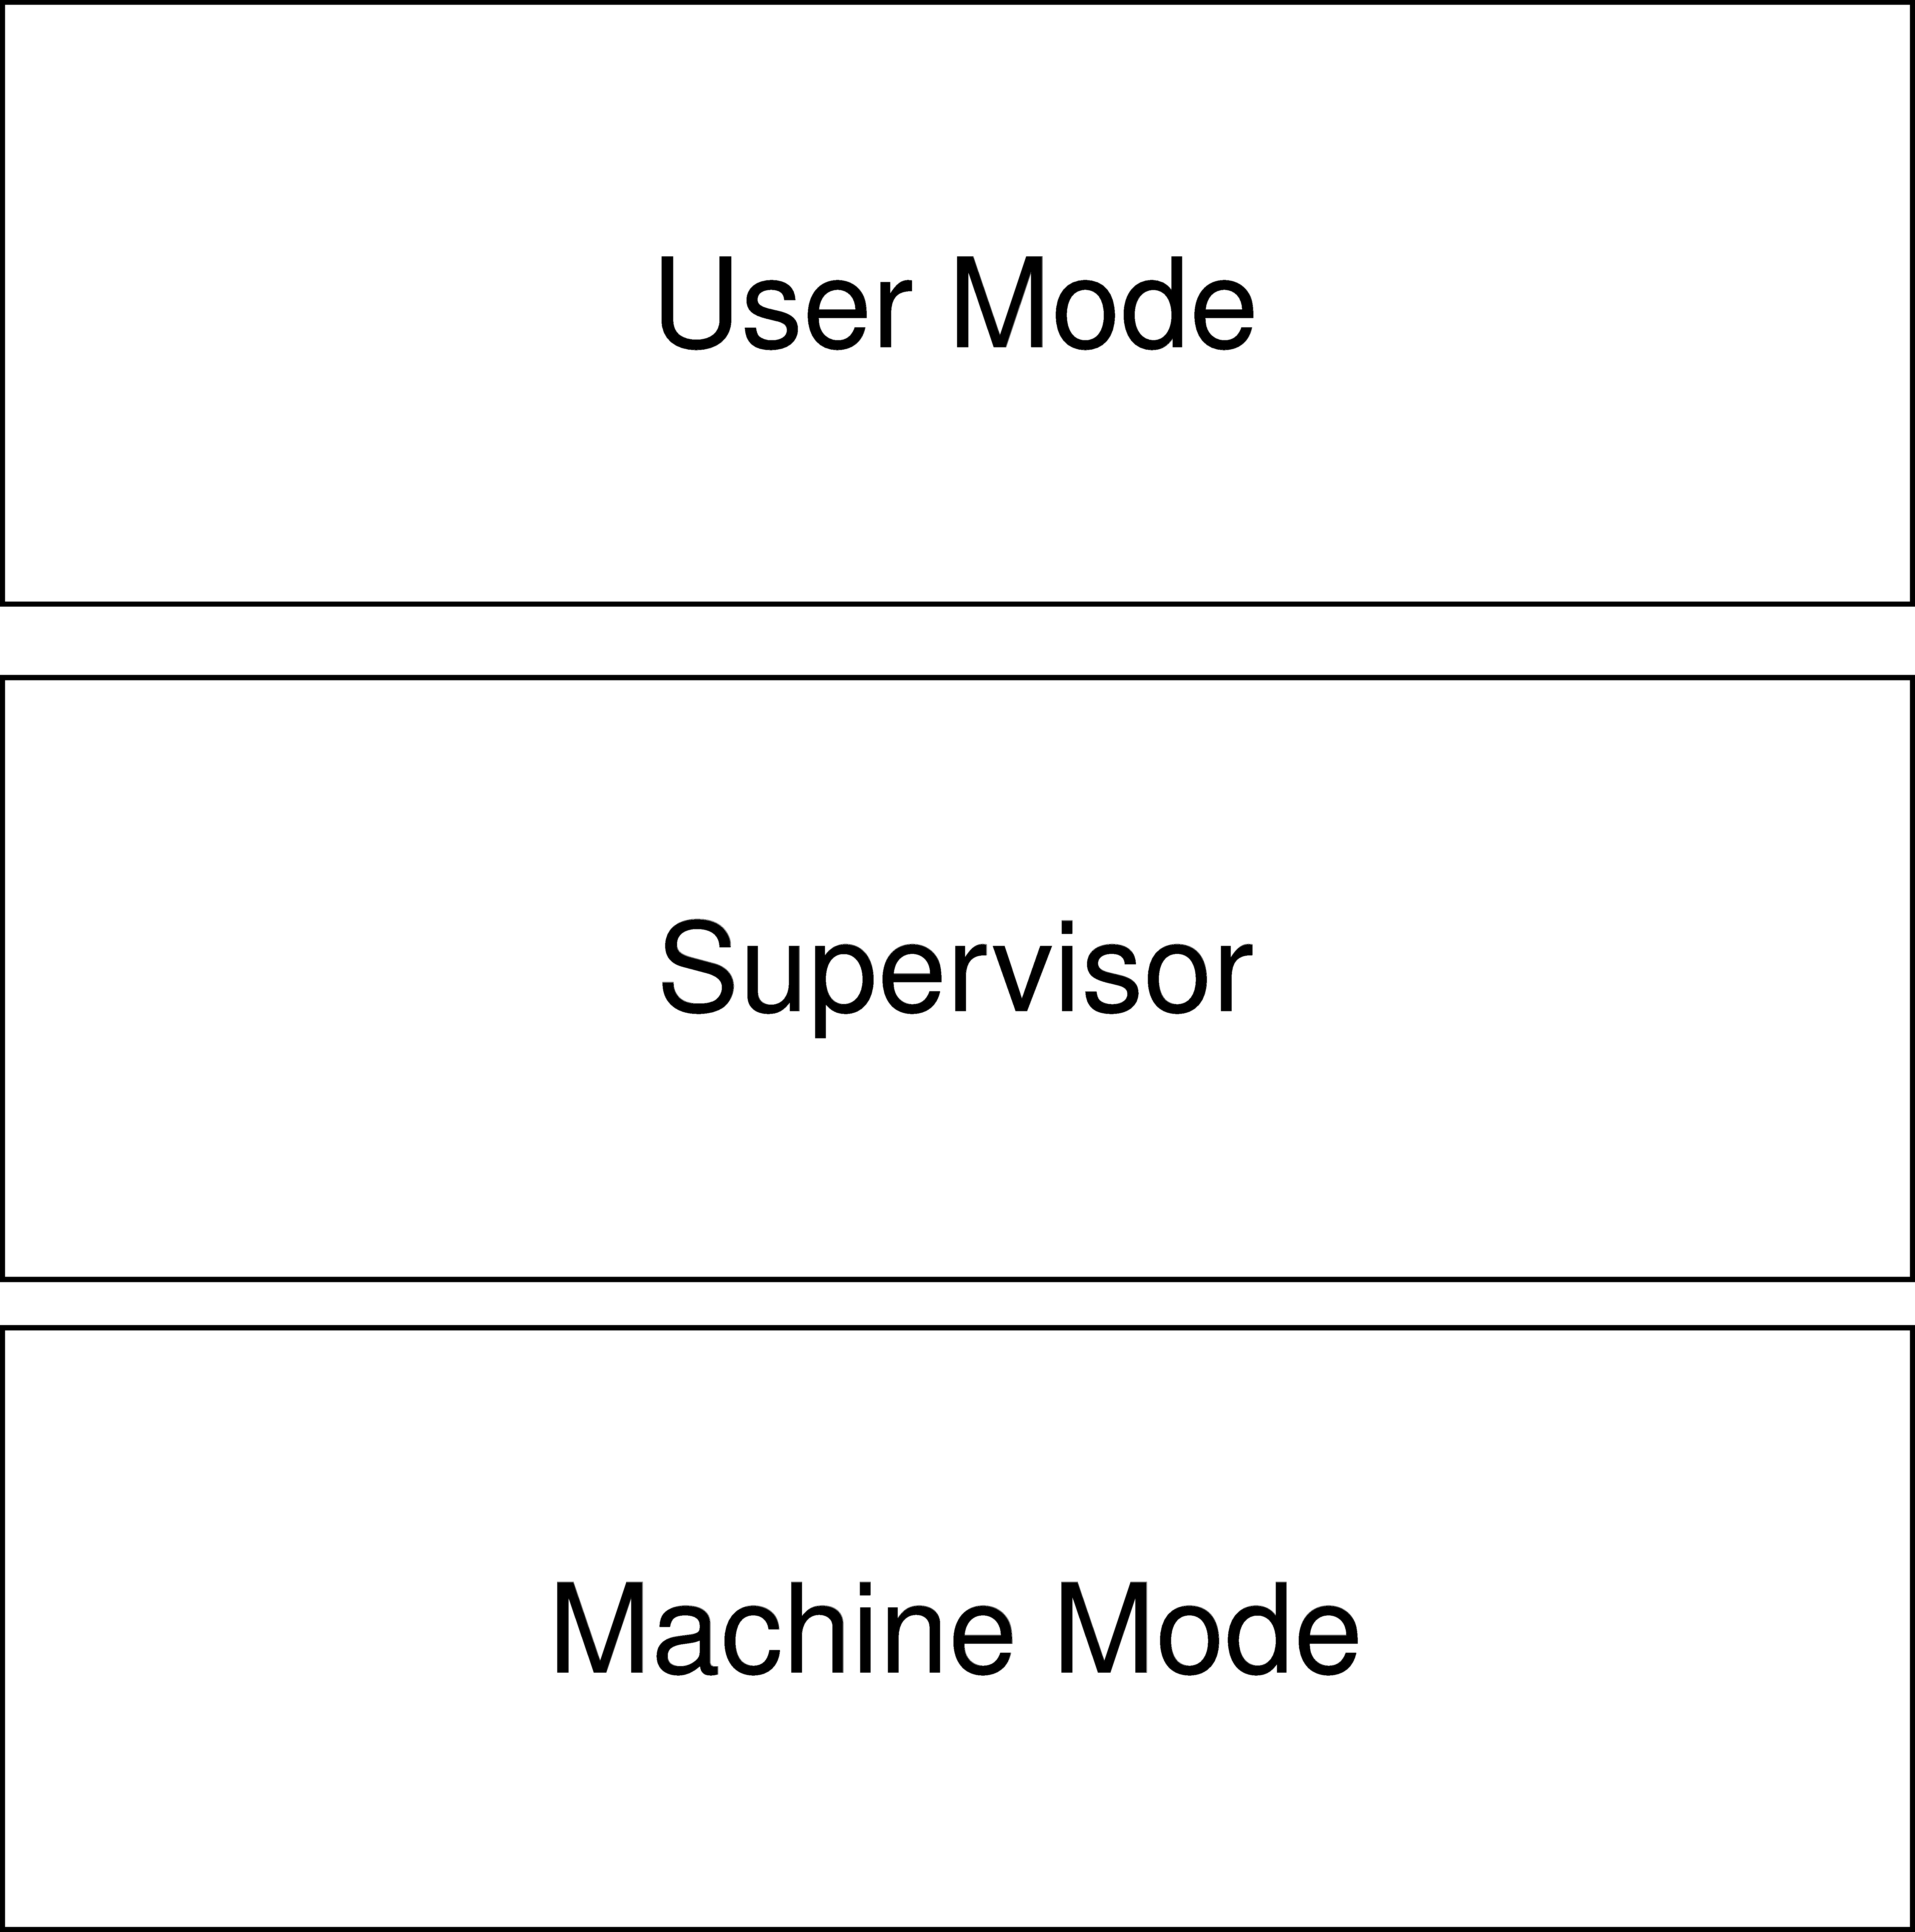
\includegraphics[width=0.3\textwidth]{images/SupervisorMode.pdf}
    \caption{Arquitetura de Privilégios RISC-V Com Modo Supervisor}\label{fig:machine-mode-user-mode-supervisor-mode}
    \end{figure}

\item \textbf{Com a extensão H:} Introduz o suporte aos modos \textit{Virtual User} e \textit{Virtual Supervisor}, estendendo os modos de privilégio para permitir a execução de hipervisores modernos.
    \begin{figure}[H]
    \centering
    \includegraphics[width=0.3\textwidth]{images/HypervisorMode.pdf}
    \caption{Arquitetura de Privilégios RISC-V Com Extensão H}\label{fig:riscv-hypervisor-mode}
    \end{figure}

\end{itemize}

\subsection{Registradores de Controle}

Os \glspl{csr} são registradores especiais utilizados para controlar e monitorar o funcionamento do processador. Eles armazenam informações essenciais relacionadas
ao estado da máquina, ao tratamento de exceções e interrupções, à configuração de privilégios e ao controle de funcionalidades específicas da arquitetura.

Esses registradores são organizados de forma segregada por nível de privilégio, sendo que cada nível dispõe do seu próprio conjunto de \glspl{csr}.
Esse isolamento é fundamental para a segurança e a integridade do sistema, pois garante uma política rígida de acessibilidade: um nível de privilégio só
pode acessar seus próprios registradores ou aqueles pertencentes a níveis menos privilegiados. Qualquer tentativa de acesso indevido a um \gls{csr} de um nível mais privilegiado 
resulta em uma exceção de instrução ilegal, impedindo que código menos privilegiado interfira diretamente nas camadas críticas do sistema.

Os principais \glspl{csr} são:

\begin{itemize}
    \item \texttt{mhartid}: mantém o identificador único de cada núcleo da CPU;\@
    \item \texttt{mstatus} e \texttt{mstatush}: mantêm os principais bits de configuração relacionados à arquitetura;
    \item \texttt{mtvec}: armazena o endereço base do vetor de manipuladores de exceções e interrupções no modo \textit{Machine};
    \item \texttt{mepc}: guarda o endereço da instrução que causou a exceção ou interrupção no modo \textit{Machine};
	\item \texttt{mcause}: armazena a causa de uma instrução ou exceção no modo \textit{Machine};
    \item \texttt{mtval}: armazena dados adicionais de uma exceção no modo \textit{Machine};
    \item \texttt{mscratch}: registrador temporário de rascunho usado para salvar ponteiros de contexto durante manipuladores no modo \textit{Machine};
    \item \texttt{mideleg} e \texttt{medeleg}: configuram a delegação de interrupções e exceções do modo \textit{Machine} para modos de menor privilégio;
    \item \texttt{mip}: mantém as interrupções atualmente pendentes;
    \item \texttt{mie}: mantém as interrupções atualmente habilitadas;
    \item \texttt{sstatus}: versão restrita e visível do registrador de status para o modo \textit{Supervisor};
    \item \texttt{stvec}: armazena o endereço base do manipulador de \textit{traps} no modo \textit{Supervisor};
    \item \texttt{sepc}: guarda o endereço da instrução que causou a exceção ou interrupção no modo \textit{Supervisor};
    \item \texttt{scause}: armazena a causa da interrupção ou exceção no modo \textit{Supervisor};
    \item \texttt{stval}: guarda informações adicionais relativas à exceção ocorrida no modo \textit{Supervisor};
    \item \texttt{sscratch}: registrador de rascunho temporário do modo \textit{Supervisor};
    \item \texttt{sip}: correspondente do modo \textit{Supervisor} ao \texttt{mip};
    \item \texttt{sie}: correspondente do modo \textit{Supervisor} ao \texttt{mie};
    \item \texttt{satp}: controla a tradução de endereços virtuais e a paginação da memória no modo \textit{Supervisor}.
\end{itemize}

\subsection{\gls{clint}}

O \gls{clint} é o mecanismo responsável por gerenciar interrupções locais — especificamente as de software e de temporização — em plataformas RISC-V.

Para a gestão de tempo, o \gls{clint} possui dois registradores centrais: \texttt{mtime} e \texttt{mtimecmp}. O \texttt{mtime} funciona como a referência temporal principal da arquitetura,
mantendo o \gls{so} ciente da passagem do tempo. O \texttt{mtimecmp}, por sua vez, determina o momento em que uma interrupção de temporização deve ser disparada:
quando o valor de \texttt{mtime} torna-se maior ou igual ao de \texttt{mtimecmp}, o \gls{clint} sinaliza o bit de interrupção temporal no registrador \gls{mip}.

Em relação às interrupções de software, o \gls{clint} disponibiliza um registrador \gls{msip} mapeado em memória para cada núcleo. Dessa forma, um núcleo pode disparar
uma interrupção de software em outro ativando o bit zero do registrador \gls{msip} pertencente ao núcleo de destino.

\subsection{\gls{plic}}

O funcionamento do \gls{plic} baseia-se na centralização e priorização de solicitações provenientes de periféricos externos. Quando uma interrupção atende aos requisitos
de habilitação e ao limiar de prioridade, o \gls{plic} notifica o núcleo ativando o bit correspondente de interrupção externa no registrador \gls{mip}, como \gls{meip} ou \gls{seip}.
A partir dessa notificação, para identificar e tratar a interrupção, o \gls{so} deve se comunicar ativamente com o \gls{plic}.

\subsection{Gerenciamento de Memória Virtual} 

A \gls{mmu} na arquitetura RISC-V é responsável por realizar a tradução de endereços virtuais em endereços físicos e por verificar as permissões de acesso à memória.
O mecanismo de tradução utilizado pelos sistemas operacionais é configurado por meio do registrador de controle \gls{satp}, disponível no modo \textit{Supervisor}.

Seu funcionamento baseia-se na paginação da memória, na qual os endereços virtuais são divididos em páginas, tipicamente com granularidade de 4,KiB. O \gls{so}
mantém tabelas de páginas que associam essas páginas virtuais a regiões da memória física e definem as permissões de acesso, como leitura, escrita e execução.
Dessa forma, quando um processo acessa um endereço virtual, a \gls{mmu} realiza a tradução correspondente e verifica se a operação solicitada é permitida.
Caso o endereço não esteja mapeado ou a operação viole as permissões estabelecidas, ocorre uma exceção de acesso à memória.

\subsection{Proteção de Memória Física}

Em sistemas que não possuem o modo supervisor --- ou como camada adicional de segurança ---, a arquitetura RISC-V emprega o mecanismo de \gls{pmp}.
Exclusivamente no modo \textit{Machine}, o firmware configura os registradores de \gls{pmp} para delimitar quais regiões da memória física podem ser acessadas pelos modos
\textit{User} e \textit{Supervisor}, assegurando o isolamento por hardware mesmo na ausência ou antes da inicialização de uma \gls{mmu}.

Para gerenciar essas regras, o mecanismo baseia-se em dois tipos de registradores: os registradores de configuração --- \textit{pmpcfg}, que definem as permissões de
acesso --- leitura, escrita e execução, o modo de pareamento de endereços e o bit de travamento para cada entrada; e os registradores de endereço --- \textit{pmpaddr},
que armazenam os endereços de referência ou parâmetros empregados pelo hardware para delimitar o tamanho e os limites das regiões protegidas.

O mecanismo de \gls{pmp} definido pela \gls{isa} da RISC-V possui três modos ativos de pareamento de endereços:

\begin{itemize}
    \item \textbf{\gls{tor}:} define uma faixa contínua de memória onde o registrador $\textit{pmpaddr}_i$ atua como o limite superior --- exclusivo --- e
        o registrador anterior $\textit{pmpaddr}_{i-1}$ atua como o limite inferior --- inclusivo. Para a primeira entrada ($i=0$), o limite inferior é considerado o
        endereço \textit{0$\times$0};
    \item \textbf{\gls{na4}:} mapeia um bloco fixo de exatamente 4 bytes apontado diretamente pelo registrador \textit{pmpaddr};
    \item \textbf{\gls{napot}:} define blocos com tamanhos que são potências de 2. O tamanho e o alinhamento da região são codificados nos bits menos significativos do próprio registrador \textit{pmpaddr}.
\end{itemize}

\subsection{Extensão H}

A extensão H introduz suporte nativo à virtualização em nível de hardware na arquitetura RISC-V. O principal objetivo dessa extensão é permitir a execução eficiente de um \gls{vmm}.
Para viabilizar esse isolamento e controle, a extensão H expande o modelo de privilégios da arquitetura, adicionando novos modos de execução:

\begin{itemize}
    \item \textbf{Virtual User:} modo no qual rodam as aplicações de usuário dentro do convidado.
    \item \textbf{Virtual Supervisor:} modo no qual o \gls{so} convidado é executado.
    \item \textbf{Hypervisor:} modo supervisor estendido, onde o hipervisor opera para gerenciar os recursos das \glspl{vm}.
\end{itemize}

\subsubsection{Tradução de Endereços em Dois Estágios}

Além dos novos modos de privilégio, a extensão H adiciona uma camada de tradução de memória para suportar a virtualização. Como múltiplos \glspl{so} convidados dependem da \gls{mmu} da plataforma
--- que normalmente seria controlada apenas pelo hipervisor ---, a arquitetura introduz os registradores \textit{vsatp} e \textit{hgatp} --- substitutos e complementos ao registrador padrão
\textit{satp} ---. Isso viabiliza uma tradução de endereços em dois estágios: o \textit{vsatp} mapeia os endereços virtuais do convidado para endereços físicos intermediários, enquanto o \textit{hgatp}
traduz esses endereços intermediários para a memória física real da máquina.

\begin{figure}[H]
\centering
\includegraphics[width=0.3\textwidth]{images/TwoStageMMU.pdf}
\caption{Tradução de Endereços em Dois Estágios da Extensão H}\label{fig:two-stage-mmu}
\end{figure}





\chapter{Trabalhos Correlatos}

\section{EPOS}

O \gls{epos}~\cite{epos-paper} é um \gls{so} de tempo real orientado a objetos, desenvolvido em C++ e voltado para sistemas embarcados e aplicações dedicadas. Seu desenvolvimento fundamenta-se
na metodologia \gls{adesd}, que busca automatizar a construção de sistemas a partir dos requisitos específicos de cada aplicação. Essa abordagem permite especializar o sistema para cenários
concretos de execução, incorporando apenas os componentes estritamente necessários e eliminando \textit{overheads} e consumo desnecessários de recursos.

Uma característica central do \gls{epos} é o emprego intensivo de metaprogramação e abstrações em C++ para deslocar decisões de configuração e especialização para o tempo de compilação.
Essa estratégia possibilita a criação de componentes altamente especializados sem impor custos em tempo de execução — propriedade indispensável em sistemas embarcados com restrições severas
de recursos.

Como ilustrado na Figura~\ref{fig:epos-architecture}, a arquitetura do EPOS é organizada em modelos de classes C++, estruturadas em diferentes níveis de abstração e de responsabilidade.
Nessa hierarquia, quanto mais alto for o nível de uma classe, mais genérica e menos especializada ela se apresenta.

\begin{figure}[H]
\centering
\includegraphics[width=0.95\textwidth]{images/EPOS.pdf}
\caption{Diagrama de Blocos da Arquitetura do EPOS}\label{fig:epos-architecture}
\end{figure}

Este trabalho fundamenta-se nos princípios arquiteturais do \gls{epos}, adotando o uso de abstrações de custo nulo e a especialização em tempo de compilação para nortear o projeto da camada
de software de baixo nível. No entanto, o escopo de aplicação difere: enquanto o \gls{epos} foca na síntese adaptativa de \gls{so} e na co-síntese de hardware e software,
o presente trabalho aplica essas diretrizes ao desenvolvimento de um hipervisor \textit{bare-metal} para a arquitetura RISC-V.
Assim, em vez de sintetizar um \gls{so} sob medida para uma aplicação específica, o objetivo é fornecer uma infraestrutura de virtualização enxuta e temporalmente previsível,
capaz de isolar múltiplos sistemas operacionais e cargas de trabalho heterogêneas.




\section{\textit{Bao Hypervisor}}

O \textit{Bao}~\cite{bao-paper} é um hipervisor \textit{bare-metal} e autossuficiente projetado para sistemas embarcados de criticidade mista. De modo análogo à solução proposta neste
trabalho, o \textit{Bao} opera de forma independente de um \gls{so} hospedeiro. No entanto, ele baseia-se em suporte dedicado de hardware, exigindo a extensão H da arquitetura RISC-V,
além de empregar um particionamento estático rígido de recursos. Em contrapartida, o hipervisor desenvolvido nesta pesquisa viabiliza a virtualização mesmo sem a extensão H
e introduz o suporte a \textit{time-sharing}, permitindo o compartilhamento temporal de núcleos de processamento entre diferentes domínios.


\section{Miralis}

O Miralis~\cite{miralis} adota uma abordagem alternativa ao empregar mecanismos computacionais semelhantes aos deste trabalho para estabelecer uma camada posicionada abaixo do firmware.
A premissa central do Miralis fundamenta-se na constatação de que raramente os fabricantes disponibilizarão firmwares formalmente verificados para o modo de máquina.
Para mitigar essa vulnerabilidade, o Miralis rebaixa a execução do firmware tradicional para o modo usuário, mantendo uma interface segura, padronizada e formalmente verificada no nível mais
privilegiado. Para isso, utiliza puramente o mecanismo de \textit{trap-and-emulate} a fim de interceptar e emular com segurança as instruções privilegiadas.
Adicionalmente, o Miralis é capaz de emular a extensão de hypervisor via software de forma transparente, viabilizando a execução de hipervisores como o Bao~\cite{bao-paper}
mesmo em plataformas desprovidas desse suporte em hardware.


\section{HSP-V}

O HSP-V~\cite{hsp-v} combina os domínios do OpenSBI com a \gls{pmp} para prover ambientes de execução isolados em processadores RISC-V.
De maneira semelhante a este trabalho, o HSP-V permite a execução de múltiplos \glspl{so} em uma mesma plataforma de hardware, mesmo na ausência da extensão H.

Além do isolamento de memória, a pilha de \textit{software} do HSP-V oferece mecanismos como o particionamento e injeção direta de interrupções, particionamento de \textit{cache} e
isolamento em nível de plataforma para dispositivos com suporte a DMA.~Contudo, o HSP-V é classificado por seus criadores como \textit{Hypervisor-Less}. Por essa razão, ele não implementa uma camada de emulação nem mecanismos para o compartilhamento ou multiplexação
de periféricos, restringindo a arquitetura à atribuição estática e exclusiva de dispositivos entre os domínios.

%Ao basear-se em mecanismos de particionamento de memória impostos por hardware, essa abordagem alcança fortes garantias de isolamento com baixo \textit{overhead} em tempo de execução.
%No entanto, diferentemente de soluções de virtualização completa, o HSP-V não implementa uma camada de hipervisor completa capaz de gerenciar e multiplexar recursos de hardware entre múltiplos
%ambientes. Consequentemente, recursos como processadores e dispositivos periféricos não podem ser compartilhados ou realocados dinamicamente entre domínios isolados, limitando a flexibilidade do sistema.



